\section{Motivation}
\label{s:challenge}

\subsection{Cloud-Native Apps and the Issues}

Cloud-native applications are usually deployed in a \emph{Pod}, which is a multi-container abstraction in Kubernetes and other platforms.
We classify cloud-native \emph{containers} into two types: infrastructure container (infra-container) and user-container, as shown in Fig.\ref{fig:motiv-cloud-native-platform}-a.
A promising benefit of cloud-native apps over non-cloud-native apps is that, \emph{cloud-native apps are developed with the supports of huge cloud infrastructure services}, including storage, network, security, etc.
For example, Envoy~\cite{envoy} is usually deployed as a infra-container by cloud vendors for each microservice (user-container) to manage network.
We highlight two issues (\textbf{I}) in nowaday cloud-native systems with such architecture.

\myparagraph{I1: Infrastructure containers bring significant burden on both CPU and memory.}
First, infra-containers introduce non-trivial resource burden.
For example, service mesh~\cite{service-mesh} is a popular pattern to manage microservices with a dedicated proxy, \emph{sidecar-proxy}, to handle network traffic on the behalf of the apps (Fig.\ref{fig:motiv-cloud-native-platform}-a).
We use the emoji-voting~\cite{emojivote} microservice to evaluate the resource costs introduced by sidecar containers on Kubernetes (detailed settings in \textsection\ref{s:case-mesh}).
Results show that proxy containers can consume up to 25\% of the CPU and 33\% of memory resources of a node.
%as shown in Fig.\ref{fig:motiv-results}-a.
Furthermore, proxy containers can consume a lot of resources even when RPS is low (RPS=20), which exacerbates resource interference further in a node.

\myparagraph{I2: Communication latency becomes more important for modular cloud-native apps.}
Microservice and serverless both are fine-grained and modular apps --- an app can be divided into tens to thousands of microservices or functions.
They rely on communication mechanism to cooperate.
As each service only takes few miliseconds for execution, the communication latency is important for end-to-end performance.
In fact, infra-containers like sidecar proxy can even increase the latency --- the latency can increase by 9.5x (RPS=20)--49.8x (RPS=3K) with proxy (Envoy)~\cite{10.1145/3620678.3624785}.
To avoid the costs, a common practice nowaday is to deploy a function chain (or highly related microservices) in the same node, and rely on local communication methods, e.g., IPC or domain socket, to reduce the latency~\cite{jianightcore, 10.1145/3503222.3507732, 273833, akkus2018sand}.
This leads to an important requirement, \emph{increasing the density of user apps, the higer the better.}
However, because of the interference of infra-containers, it is hard.

\begin{figure}[t]
\setlength{\belowcaptionskip}{-10pt}
\setlength{\abovecaptionskip}{0pt}
  \centering 
  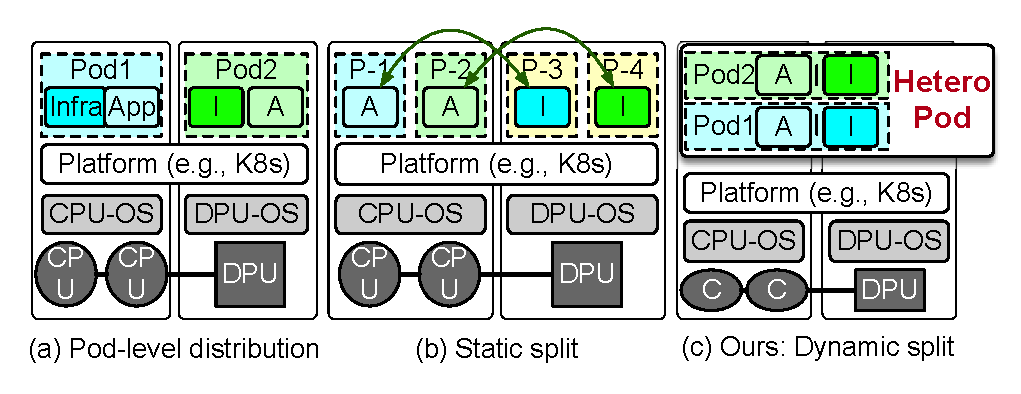
\includegraphics[width=0.48\textwidth]{figs/intro-cloud-native-issue.eps}
  \footnotesize %\\[-5pt]
  \caption{\textbf{Cloud-native apps on CPU-DPU computers.}
  }
  \label{fig:intro-issue}
\end{figure}


\subsection{CPU-DPU Platforms for Cloud-Native Apps}
\label{s:dpu}

DPUs (data processing units)~\cite{netronomeagilio, mellanoxbf, marvel-octeon-sdk} are a new class of programmable devices that move and process data around the data centers.
It is an SoC and capable of running commercial OSes and performance-critical programs like network proxy.
DPU usually includes multi-core processing unit (e.g., 2.75GHz ARM cores in Bluefield-2 DPU) and efficient network interface.
Prior works have shown that DPU can improve the density of serverless functions~\cite{10.1145/3503222.3507732}, reduce the latency and resource costs for DFS~\cite{10.1145/3477132.3483565}, and enable energy-efficient microservices~\cite{234944}.

\myparagraph{Efforts using DPU for cloud-native apps.}
Commercial cloud platforms commonly use either 
\emph{pod-level distribution}, e.g., NVIDIA DPU Container~\cite{nvidia-doca-container} and Red Hat OpenShift~\cite{redhat-openshift},
or \emph{static split}~\cite{10.1145/3477132.3483565, li2020leapio, seshadri2014willow}, e.g., Azure~\cite{firestone2018azure},
as shown in Fig.\ref{fig:intro-issue}-a/b.
Pod-level distribution treats DPUs as individual servers and deploy unmodified apps directly on the DPUs.
However, apps may suffer significant performance degradation 
due to mismatches between their requirements and the hardware capabilities, e.g., a DPU usually has wimpy cores.
On the other hand, static split involves breaking down an app into fine-grained components that can be distributed across different PUs, leveraging communication for cooperation.
This approach can deliver great performance by deploying only suitable components on DPUs, such as computation-intensive components on CPU and network-intensive components on DPU.
However, this method typically requires an understanding of apps and hardware during development, making it challenging to adapt for generic apps and heterogeneous devices.
Despite these limitations, both methods are practical and can offer specific benefits in real-world industry apps.

Recent research efforts have led to the development of new heterogeneous frameworks for specific cloud-native scenarios, e.g., serverless computing~\cite{10.1145/3503222.3507732} and microservices~\cite{234944}.
However, these frameworks usually require app modifications, which limit their ability to support only simple apps (less than 1.8K lines of Node.js code in Molecule~\cite{10.1145/3503222.3507732}) and are \emph{not practical enough} for complex commodity applications like Envoy (a widely used service mesh proxy with 764K lines of C++ code).
This is a significant limitation given that many commodity cloud-native apps are distributed in binary or container image format, making it difficult to modify them.


\myparagraph{Our approach: dynamic split with \xpod.}
%In contrast to co-locating infrastructure and app containers on host CPUs and prior CPU-DPU systems,
In contrast to prior methods, %co-locating infrastructure and app containers on host CPUs and prior CPU-DPU systems,
we propose \emph{dynamic cross-PU decoupling} --- transparently partitioning containers (even from the same Pod) across heterogeneous PUs during runtime,
as illustrated in Fig.~\ref{fig:intro-issue}-c. This architecture, termed \xpod (Cross-PU Pod), addresses critical limitations of conventional deployments.
First, isolating infrastructure containers on DPUs eliminates resource contention with application containers.
Second, DPU can help improve the density of a single node by also offloading suitable user-containers to DPU.
Last and also most important, unlike the static split approach, \xpod's dynamic split preserves existing Pod semantics, supporting unmodified commodity cloud-native apps.

